\documentclass[10pt,letterpaper]{article}
\usepackage[margin=0.85in]{geometry}
\usepackage{amsmath,booktabs,graphicx,xcolor}
\usepackage[hidelinks]{hyperref}

\definecolor{reviewred}{RGB}{153,24,30}
\newif\ifreview
\reviewfalse
\newcommand{\reviewcolor}{\ifreview\color{reviewred}\fi}
\newcommand{\reviewtext}[1]{{\reviewcolor #1}}
\newenvironment{reviewedit}{\reviewcolor}{}
\setlength{\parindent}{0pt}
\setlength{\parskip}{0.42\baselineskip}
\setlength{\emergencystretch}{1.5em}
\title{\vspace{-1.2em}Adaptive Video Bitrate Selection\\under Varying Network Conditions}
\author{CSE 250A Final Project\\Boqi (Bobby) Zhu, Hanyue Zhang, Qinchuan Zhang, and Xin Chen}
\date{}

\begin{document}
\maketitle
\vspace{-1.5em}

\section{Problem Description}

An adaptive bitrate (ABR) player selects the quality of each video chunk before
downloading it. A higher bitrate improves picture quality, but a slow download
can empty the playback buffer and cause a stall. Large changes between
successive bitrates also carry a cost. We ask whether a tabular Q-learning
policy can use recent download measurements to improve Quality of Experience
(QoE) relative to a fixed-rate policy and a policy that uses buffer occupancy
alone. We also examine which playback costs account for the observed gains
and losses.

\section{Data Sourcing and Processing}

We used 428 FCC and HSDPA bandwidth traces from the public trace
repository~\cite{traces}. Each file contains timestamps and bandwidth in Mbit/s.
We retained zero-bandwidth intervals to represent outages. MERINA provided the
chunk sizes for one video, Mao, with 49 four-second chunks at each of six
bitrates~\cite{merina}.

The imported training partition contained 166 files. The imported holdout set
contained 262 slices from 39 longer recordings. An early split by file placed
slices from 36 recordings in both validation and test. We corrected this by
allocating whole recordings within each source using a deterministic rule
based on a hash of the recording identifier. The resulting manifests contain
166 training, 129 validation, and 133 test files with no recording identifiers
shared across splits. The test files represent only 20 recordings, including
six FCC and 14 HSDPA recordings~\cite{splits}. This matters because adjacent
slices from the same recording can share network conditions.

\begin{reviewedit}
We also checked the 166 training files against all 131 original validation
files and then against all 129 revised validation files. In both versions
we found zero shared filename-derived recording IDs, zero identical full
bandwidth sequences, and zero exact matches of a 16-sample bandwidth window
containing at least two distinct values. Comparing the bandwidth values at
any offset allows timestamps to differ. Resampled copies could escape these
checks. In the original validation--test split, 119 of 131 test slices had
a sibling from the same recording in validation. In the revised split this
count was zero of 133. The audit describes the main experiment's partitions.
Of its 20 test recording IDs, 14 appeared in training and two in validation
in an earlier exploratory prototype with a separate partition~\cite{prototype}.
\end{reviewedit}

\section{Modeling and Inference}

\paragraph{Environment and reward.}
We used one trace-driven simulator for all policies. The download delay
depends on the selected chunk size and the bandwidth available over its
transfer, with 95\% payload efficiency and 80 ms RTT. Playback drains the
buffer during transfer. Time spent with an empty buffer counts as
rebuffering, and a completed download adds four seconds of playback. The
simulator can wrap to the start of a trace when it reaches the end. For
selected bitrate \(b_t\) in Mbit/s and rebuffering duration \(u_t\) in seconds,
the per-chunk reward is
\[
r_t=b_t-4.3u_t-\lvert b_t-b_{t-1}\rvert.
\]
The simulator uses \(b_0=0.75\) Mbit/s for all policies. QoE per video is the sum
of rewards across all 49 chunks~\cite{simulator}.

\paragraph{State, action, and learning.}
Before selecting a bitrate, the agent observes a bin for the harmonic mean of
the most recent three completed-download throughputs, a bin for the current
buffer, and the previous bitrate index. The throughput features use only
completed downloads, with a separate bin before the first download. The
selected discretization has 486 states. The action ladder is 300, 750, 1200,
1850, 2850, or 4300 kbps. We update the table with
\[
 Q(s,a)\gets Q(s,a)+\alpha\left[r+\gamma\max_{a'}Q(s',a')-Q(s,a)\right],
\]
with a target of \(r\) at the final chunk.

Each training episode plays the full video from a random position in a
randomly sampled training trace. Exploration uses an \(\epsilon\)-greedy
policy, with \(\epsilon\) decreasing linearly from 1.0 to 0.01 over the first
80\% of training. A two-round validation search compared discretization,
learning rate, discount, history length, and training schedules. The
selected setting used fine bins, \(\alpha=0.02\), \(\gamma=0.5\), and 30,000
episodes. We retrained that setting with five fresh seeds (100--104) and
evaluated the frozen greedy policies from the beginning of each test trace.

\paragraph{Baselines.}
The fixed policy selects 1200 kbps for every chunk. The buffer-based rule
uses a 10-second reservoir and a 40-second cushion to map buffer occupancy
to a bitrate. The baselines use their declared defaults~\cite{implementation}. Section~4
also reports a buffer rule tuned on validation as a robustness check.

\section{Results and Discussion}

\begin{table}[htbp]
\centering
\small
\caption{Test results across 133 trace files. Q-learning entries show mean
\(\pm\) standard deviation across five training seeds.}
\label{tab:test}
\begin{tabular}{lrrrr}
\toprule
Policy & QoE/video & Bitrate (kbps) & Rebuffer (s/video) & Switches/video \\
\midrule
Fixed 1200 kbps & \(-261.37\) & 1200 & 74.35 & 1.00 \\
Buffer-based & \(36.78\) & 1069 & 1.66 & 14.48 \\
Q-learning & \(39.64\pm1.10\) & \(1176\pm7\) & \(1.97\pm0.11\) & \(12.34\pm1.95\) \\
\bottomrule
\end{tabular}
\end{table}

Q-learning improved average test QoE by 2.86 points over the buffer-based
baseline. \reviewtext{Giving each original recording equal weight produced a similar
gain of 2.76 points.} The table reports variation across training seeds.
\reviewtext{To estimate uncertainty across recordings, we first averaged
the five agents' QoE on each slice and subtracted the buffer baseline on that
slice. We resampled the 20 original recordings with replacement 10,000 times
and averaged the slice differences in each draw, keeping sibling slices
together. The 95\% percentile interval for the 2.86-point gain was
\([0.20, 5.98]\) QoE points per video.} The fixed-rate policy incurred over a minute of
stall time per video on average, consistent with its inability to lower the
rate when the connection cannot sustain 1200 kbps~\cite{testresults}.

The default buffer rule was not tuned. We therefore searched its reservoir
(0--15 s) and cushion (10--50 s) on validation only. The best setting, a
10-second reservoir and 25-second cushion, scored 44.97 on validation against
43.94 for the default and 37.19 on test against 36.78. Q-learning's advantage
over this tuned rule was 2.45 points, with a paired recording-bootstrap
interval of \([0.15, 5.01]\). Section~\ref{sec:learned} explains why tuning
the buffer thresholds closes little of the gap.

\begin{reviewedit}
\subsection{What Accounts for the QoE Gain?}

The reward breakdown explains why a policy with more rebuffering can still
score higher. Across all test traces, the higher bitrates added 5.25 QoE
points per video. Additional stalls cost 1.34 points, and larger cumulative
bitrate changes cost 1.05 points. Q-learning made fewer switches on average
(Table~\ref{tab:test}), yet the sum of their magnitudes was higher, and the
smoothness term penalizes that sum. The buffer rule climbs its linear ramp one
rung at a time, so only 3.3\% of its switches exceeded 1000 kbps. Q-learning's
action follows the throughput bin, and 19.1\% of its switches exceeded
1000 kbps.

\begin{table}[htbp]
\reviewcolor
\centering
\small
\caption{Q-learning minus buffer-based QoE per video, decomposed into
signed contributions. The components are rounded independently.}
\label{tab:decomposition}
\begin{tabular}{lrrrr}
\toprule
Test subset & Bitrate & Rebuffering & Switching magnitude & Total \\
\midrule
FCC (45 slices) & \(+5.99\) & \(-0.59\) & \(+0.76\) & \(+6.16\) \\
HSDPA (88 slices) & \(+4.88\) & \(-1.72\) & \(-1.98\) & \(+1.18\) \\
All (133 slices) & \(+5.25\) & \(-1.34\) & \(-1.05\) & \(+2.86\) \\
\bottomrule
\end{tabular}
\end{table}

The gain from selecting higher rates appeared in both networks
(Table~\ref{tab:decomposition}). The difference was how much each policy paid
for that gain. On FCC, the rebuffer cost was small and the switching term
favored Q-learning. On HSDPA, rebuffering and switching costs absorbed most
of the higher-bitrate reward. Resampling whole recordings within each source
gave a 95\% interval of \([-1.30, 4.26]\) for HSDPA and \([1.46, 12.02]\)
for FCC. The HSDPA mean remains uncertain, and the FCC estimate rests on
six recordings.

\subsection{What Did the Agent Learn?}
\label{sec:learned}

We replayed the five archived test agents and the buffer rule decision by
decision. The replay reproduces every committed per-slice score. In the states
Q-learning visited on test, it chose a higher bitrate than the buffer rule would
have chosen in the same state 62.7\% of the time and a lower one only 2.0\% of
the time. Figure~\ref{fig:policy}c shows the reason. With 14--19 seconds buffered,
Q-learning's mean choice rises from 341 kbps at the lowest throughput estimate
to 3730 kbps at the highest. The buffer rule stays near 400 kbps in the same
states because it does not read throughput.

\begin{figure}[htbp]
\centering
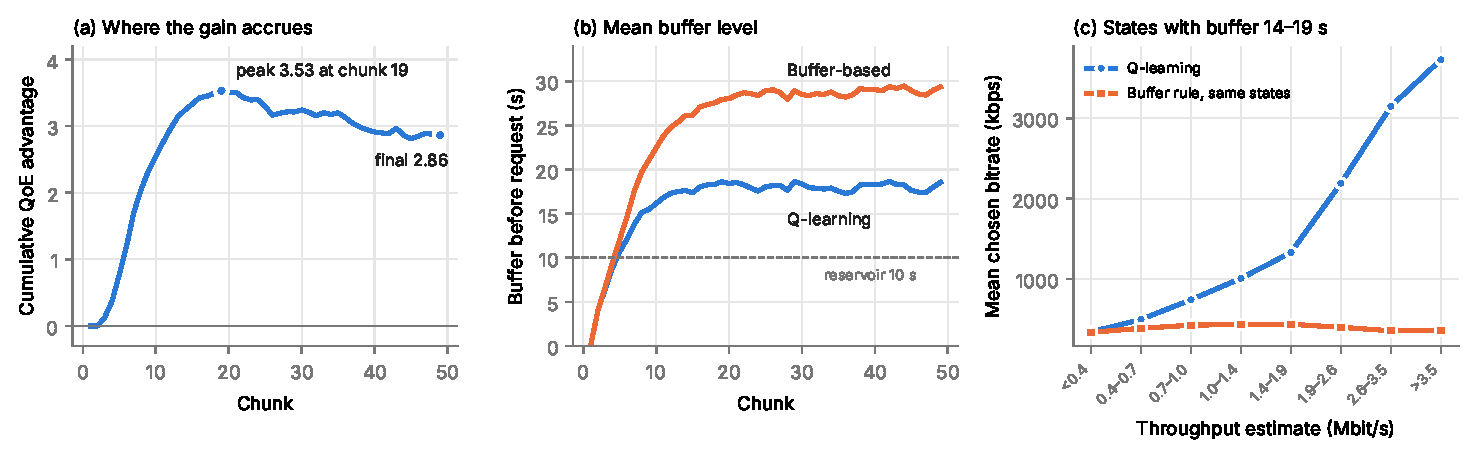
\includegraphics[width=\linewidth]{images/policy_behavior.pdf}
\caption{(a) Cumulative per-chunk QoE of Q-learning minus the buffer rule,
averaged over test slices and seeds. (b) Mean buffer before each request.
(c) Mean bitrate chosen by Q-learning in its own test states with 14--19 s
buffered, by throughput-estimate bin, and the bitrate the buffer rule assigns
to those states.}
\label{fig:policy}
\end{figure}

\textbf{The gain is concentrated in the start-up phase.} The cumulative advantage
reaches 3.53 points by chunk 19. The remaining 30 chunks give back 0.67 points net
(Figure~\ref{fig:policy}a). The buffer rule requests 300 kbps until its
10-second reservoir fills, about five chunks, and then climbs as the buffer
grows. Q-learning leaves the lowest rate as soon as measured throughput allows.
Its mean bitrate over the first ten chunks was 783 kbps, against 456 kbps.
The start-up boundary is not sharp, so the split depends on the cutoff: chunks
1--10 contribute 2.54 points and chunks 1--15 contribute 3.33. No setting of
the buffer thresholds can reproduce this behavior, because the rule never sees
throughput.

\textbf{In steady state, Q-learning holds a smaller reserve.} After start-up it
keeps about 18 seconds buffered, against about 28 for the buffer rule
(Figure~\ref{fig:policy}b). The buffer rule spends 17\% of its decisions
above 35 seconds, a level Q-learning reached in 16 of 32,585 decisions. Using
buffer for bitrate paid off on FCC, where chunks 11--49 added 3.05 points. On
HSDPA the same chunks lost 1.08 points. A larger reserve absorbs a throughput
collapse that a smaller one cannot. The selected discount of 0.5 weights only a
few chunks ahead, which may undervalue a reserve whose benefit is rare and
delayed. Shorter horizons scored higher on average in validation
(Section~\ref{sec:stability}), so the lean buffer may be a deliberate average-case
tradeoff rather than a training defect. The grid did not isolate this effect,
so it remains a hypothesis.

\textbf{Stalls follow sudden collapses, not unfamiliar states.} About 35\% of
the fine-bin states were never visited in training, but 97.8\% of test decisions fell
in states visited more than 1000 times, and none fell in an unvisited state.
States with at most 1000 visits account for 1.9\% of rebuffering. Requests
whose delivered throughput fell below half of the prior estimate were 1.8\% of
post-start decisions but caused 57\% of post-start rebuffering. On average, Q-learning
was not more aggressive relative to its estimate than the buffer rule. Both
requested more than the estimate in about a third of decisions, with the same
median ratio of 0.87. The difference is the reserve when a collapse arrives.
The chunk 39 replay in Section~\ref{sec:cases} is one such case.

\subsection{Two Outcomes Within the Same HSDPA Recording}
\label{sec:cases}

Two slices of \texttt{norway\_car\_1} illustrate how the tradeoff changes
within a single recording. We chose the pair with the largest QoE contrast
among same-recording pairs that won in one slice and lost in the other for
all five seeds. The examples illustrate failure and success modes.
On \texttt{part0}, Q-learning raised the mean bitrate from 1712 to 2013 kbps
with the same 0.56 seconds of stalling and gained 21.35 points (averaged over
the five seeds). On \texttt{part2}, it raised the mean bitrate from 981 to
1123 kbps, but stalling grew from 0.53 to 10.87 seconds and it lost 44.02
points. The higher bitrate added 7.00 points, while the extra 10.34 seconds of
stalling cost 44.44 points before the additional switching penalty.

We replayed the first archived agent (seed 100) from the beginning of
\texttt{part2}. It stalled twice after startup (Table~\ref{tab:replay}).
At chunk 10 it chose a bitrate below the harmonic mean of the three previous
downloads, yet the new download delivered just 0.31 Mbit/s. At chunk 39
the agent chose 2.85 Mbit/s with 17.72 seconds buffered. The download took
26.52 seconds, exhausting even this larger reserve. The buffer baseline
incurred only the 0.53-second startup wait on its own replay. Earlier
choices affect request timing, so the two policies can encounter different
parts of the trace when they download the same video chunk.

\begin{table}[htbp]
\reviewcolor
\centering\small
\caption{Both post-startup stalls for seed 100 on \texttt{norway\_car\_1\_part2}.
The estimate uses completed downloads before the request. Rates are in Mbit/s
and times in seconds. Chunk numbers start at 1.}
\label{tab:replay}
\begin{tabular}{rrrrrrr}
\toprule
Chunk & Prior estimate & Chosen rate & Measured rate & Buffer before & Download & Stall \\
\midrule
10 & 1.28 & 1.20 & 0.31 & 8.76 & 14.41 & 5.66 \\
39 & 2.11 & 2.85 & 0.43 & 17.72 & 26.52 & 8.80 \\
\bottomrule
\end{tabular}
\end{table}
\end{reviewedit}

\subsection{Does Throughput Predictability Explain the Source Difference?}

FCC samples are spaced five seconds apart, whereas HSDPA samples typically
arrive about once per second. To compare the same time horizon, we formed
duration-weighted five-second windows and used the harmonic mean of the
previous three windows to predict the next one. FCC had lower median
normalized forecast error (0.193 versus 0.219), while HSDPA had higher
lag-one correlation (0.405 versus 0.147). These statistics measure different
properties. Correlation measures persistence, while forecast error measures
the accuracy of a specific predictor.

Across the 133 test slices, three-window forecast error was negatively
correlated with Q-learning's QoE advantage (\(r=-0.464\)). This value pools
all test slices from both sources, while Figure~\ref{fig:forecast} reports
the correlation within each source (\(r=-0.25\) for FCC and \(r=-0.52\) for
HSDPA). The association
persisted when averaging within each of the 20 original recordings
(\(r=-0.628\)). Mean bandwidth and variability were also associated with the
gain. In addition, fixed-time link bandwidth differs from the actual chunk
throughput measured by the agent. These slice-level associations agree with the
decision-level replay in Section~\ref{sec:learned}: most post-start
rebuffering followed downloads much slower than the agent's estimate, and
such surprises are more frequent where throughput is harder to forecast. Both
analyses are correlational. Establishing the mechanism would require
controlling for mean bandwidth and testing on more recordings~\cite{dynamics}.

\begin{figure}[htbp]
\centering
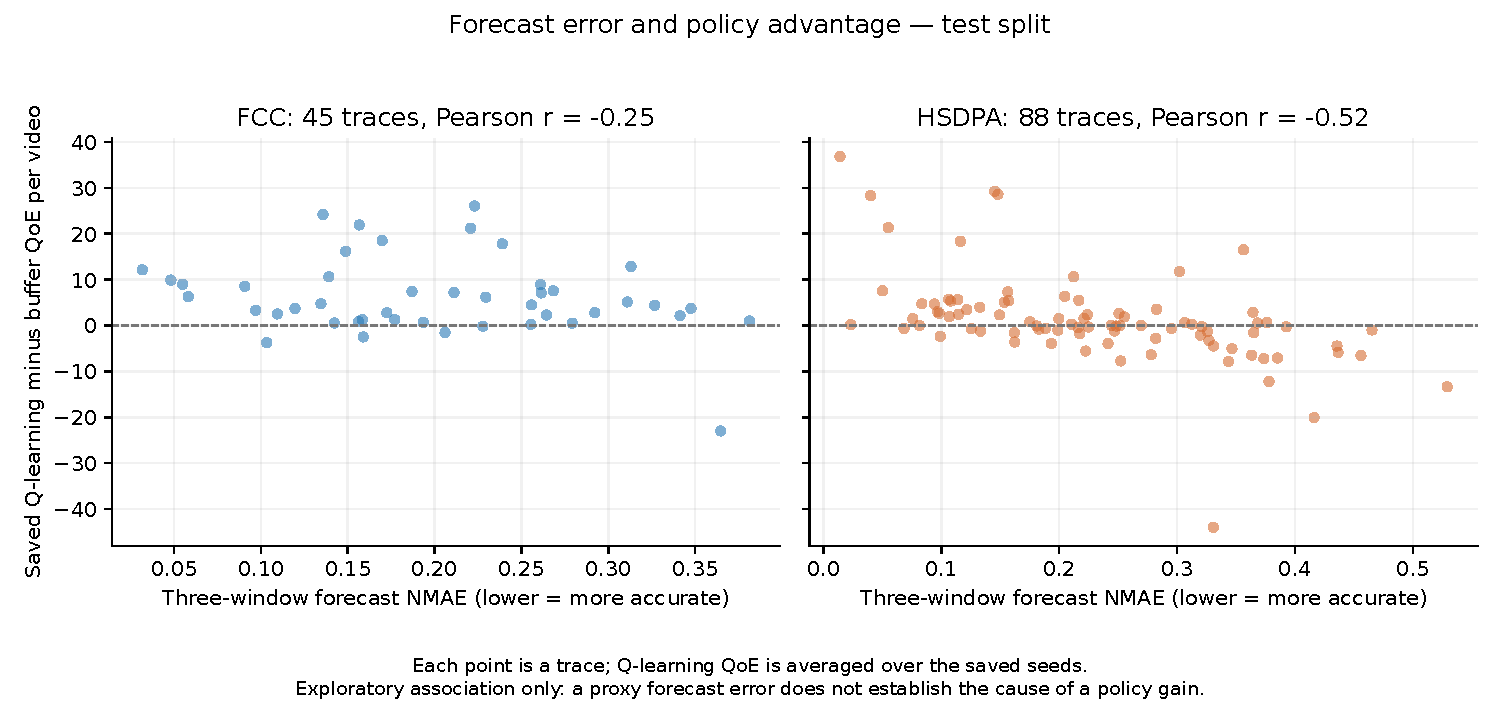
\includegraphics[width=0.72\linewidth]{images/test_qoe_relationship.pdf}
\caption{The gain over buffer-based adaptation is often larger at lower
normalized forecast error. Each point represents a test slice. Slices can
share an original recording.}
\label{fig:forecast}
\end{figure}

\subsection{Validation Stability and Scaling}
\label{sec:stability}

Fine discretization appeared throughout the top validation configurations,
and lower learning rates and shorter discount horizons performed better in
the explored grid. Several leading configurations were within roughly one
seed standard deviation, so the exact ranking is uncertain~\cite{implementation}.

\begin{reviewedit}
\paragraph{Shorter training budget:}
We trained the selected configuration for 10,000 episodes with the original
five tuning seeds (0--4) and evaluated the greedy policies on the same 129
validation traces. The exploration rate decayed over the first 80\% of each
run, and the remaining hyperparameters were held fixed. Validation QoE was
\(44.43\pm1.33\), compared with \(46.48\pm1.97\) for the archived 30,000-episode
setting (\href{https://github.com/Bobby-Zhu/abr-q-learning/blob/2169df2/results/q_learning/tuning.csv}{round-two tuning results}).
These values are the mean and sample standard deviation across seeds.
Using one third of the training episodes cost 2.05 QoE points on average.
The comparison supports keeping the 30,000-episode budget for the reported
configuration.
\end{reviewedit}

\section{Conclusion}

On the shared simulator, tabular Q-learning achieved higher average QoE than
both baselines and than a validation-tuned version of the buffer rule. The gain
came mainly from using throughput to leave the lowest bitrate early in the
video. In steady state the agent traded buffer for bitrate, which helped on
FCC and hurt on HSDPA, where sudden throughput collapses caused most of its
stalls. The evaluation used one video and a small number of source recordings.

\paragraph{Next steps.} Each follow-up targets one finding and would be
selected on validation.
(1)~Keep a reserve when throughput is volatile, by adding a variability bin to
the state or a small low-buffer penalty, and measure post-start stall time on
HSDPA.
(2)~Test whether a longer discount horizon, with more training episodes,
raises the steady-state buffer.
(3)~Restrict actions to one or two rungs from the previous bitrate to reduce
the large-jump penalty.
(4)~Combine the learned start-up behavior with a buffer rule afterwards, to
test whether the steady-state policy adds value on HSDPA.
(5)~Following the chunk 39 replay, discount the throughput estimate after sharp
fluctuations.
Finer state bins are a lower priority, because test decisions already stay in
well-visited states. More videos and recordings would strengthen every
comparison.

\section{Reflections \& Contributions}

One practical lesson from this project is to define the holdout unit before
tuning a policy. Grouping by original recording matters when successive
segments can share the same network conditions. Keeping the QoE components
alongside the total score also makes it possible to identify why a policy
wins or fails on a particular trace.

\paragraph{Boqi (Bobby) Zhu:}
I adapted MERINA's simulator and implemented the fixed-bitrate and buffer-based
policies with shared configuration, QoE evaluation, and automated tests.
I also analyzed FCC and HSDPA trace dynamics on a common five-second grid,
comparing variability, autocorrelation, and forecast errors and relating
these measurements to the saved Q-learning gains over the buffer baseline.

I learned that a plausible explanation for a performance difference needs
evidence from the data. HSDPA had higher autocorrelation but slightly larger
normalized forecast error, which taught me to distinguish temporal correlation
from prediction accuracy and to avoid treating an association as proof of a
causal explanation.

\paragraph{Xin Chen:}
I broke down the test QoE gap by reward component and compared two slices
from the same HSDPA recording to examine when Q-learning helped or hurt.
I also ran the 10,000-episode validation experiment and compared it with the
archived 30,000-episode setting using the same validation traces and seeds.

I learned to check what each reward term measures. Q-learning switched
bitrates less often than the buffer baseline, but the changes added up to a
larger switching penalty.

\paragraph{Hanyue Zhang:}
I audited the data splits and found that the holdout files were consecutive
slices of 39 longer recordings, 36 of which appeared in both validation and
test. I regrouped the holdout by recording and added a check that fails if a
recording crosses splits. I also implemented the tabular Q-learning agent,
tuned it on validation only, ran the five-seed test comparison against both
baselines, and fixed a simulator edge case where a download ending exactly on
a trace timestamp stopped the episode.

I learned that the split can matter as much as the model. Neighbouring slices
of the same trip made validation look like test, so tuning on it would have
overstated the final scores.

\paragraph{AI use.}
ChatGPT assisted with project brainstorming and proposal wording. The
merged Q-learning implementation PR records Claude Code assistance. Codex
helped check the saved results and prepare this review draft. Claude Code
assisted with the decision-level policy analysis and the tuned-baseline check.

\appendix
\section{State Bins and Reproduction}

The selected throughput bin edges in Mbit/s are 0.4, 0.7, 1.0, 1.4, 1.9,
2.6, and 3.5. The buffer edges in seconds are 2, 4, 7, 10, 14, 19, 26, and
35. Observations on an edge are assigned to the upper bin. The team
repository records the manifests, selected configuration, test outputs, and
analysis scripts at commit \texttt{2169df2}.
\reviewtext{The accompanying scripts in \texttt{docs/technical\_report/}
reproduce the split audit (\texttt{check\_splits.py}), the chunk replay
(\texttt{replay\_case.py}), and the paired bootstrap intervals
(\texttt{recording\_intervals.py}), the decision-level policy analysis and
Figure~\ref{fig:policy} (\texttt{policy\_analysis.py}), and the tuned buffer
baseline (\texttt{tuned\_buffer.py}). Each accepts \texttt{--repo} followed
by the path to the repository.}

\begin{thebibliography}{9}
\bibitem{traces}
Nuowen Kan. \emph{Real-world bandwidth traces}. MIT-licensed data repository.
\href{https://github.com/confiwent/Real-world-bandwidth-traces/tree/d28c4fd48d0e358db024cc0217b111c070815fa7}{Source and version}.

\bibitem{merina}
Nuowen Kan. \emph{MERINA}. MIT-licensed simulation code and chunk metadata.
\href{https://github.com/confiwent/merina/tree/dfd01b7f664e3a9fa0d123945081f7af2ebb31f7}{Source and version}.

\bibitem{splits}
Project team. \emph{Deterministic trace splits}.
\href{https://github.com/Bobby-Zhu/abr-q-learning/blob/2169df2/data/splits/README.md}{Split documentation} and
\href{https://github.com/Bobby-Zhu/abr-q-learning/pull/1}{recording-level split fix}.

\bibitem{simulator}
Project team. \emph{ABR simulator and reward configuration}.
\href{https://github.com/Bobby-Zhu/abr-q-learning/blob/2169df2/docs/SIMULATOR.md}{Repository documentation}.

\bibitem{implementation}
Project team. \emph{Tabular Q-learning for ABR}.
\href{https://github.com/Bobby-Zhu/abr-q-learning/blob/2169df2/docs/Q_LEARNING.md}{Training and evaluation protocol} and
\href{https://github.com/Bobby-Zhu/abr-q-learning/pull/2}{implementation PR}.

\bibitem{testresults}
Project team. \emph{Frozen test comparison}.
\href{https://github.com/Bobby-Zhu/abr-q-learning/blob/2169df2/results/final/test/summary.md}{Summary},
\href{https://github.com/Bobby-Zhu/abr-q-learning/blob/2169df2/results/final/test/per_trace.csv}{per-slice metrics}, and
\href{https://github.com/Bobby-Zhu/abr-q-learning/blob/2169df2/results/trace_dynamics/per_recording.csv}{recording-level summaries}.

\bibitem{dynamics}
Project team. \emph{Trace dynamics analysis}.
\href{https://github.com/Bobby-Zhu/abr-q-learning/blob/2169df2/docs/TRACE_DYNAMICS.md}{Methods, figures, and interpretation}.
\bibitem{prototype}
Project team. \emph{Earlier exploratory prototype}.
\href{https://github.com/Bobby-Zhu/abr-q-learning/blob/1c8251acc07a97f89b18e78ff958b8d3b061339e/prototype/results/run_01/manifest.csv}{Run manifest}.
\end{thebibliography}
\end{document}
